\newcommand{\NWtarget}[2]{\hypertarget{#1}{#2}}
\newcommand{\NWlink}[2]{\hyperlink{#1}{#2}}
\newcommand{\NWtxtMacroDefBy}{Fragment defined by}
\newcommand{\NWtxtMacroRefIn}{Fragment referenced in}
\newcommand{\NWtxtMacroNoRef}{Fragment never referenced}
\newcommand{\NWtxtDefBy}{Defined by}
\newcommand{\NWtxtRefIn}{Referenced in}
\newcommand{\NWtxtNoRef}{Not referenced}
\newcommand{\NWtxtFileDefBy}{File defined by}
\newcommand{\NWtxtIdentsUsed}{Uses:}
\newcommand{\NWtxtIdentsNotUsed}{Never used}
\newcommand{\NWtxtIdentsDefed}{Defines:}
\newcommand{\NWsep}{${\diamond}$}
\newcommand{\NWnotglobal}{(not defined globally)}
\newcommand{\NWuseHyperlinks}{}
% -*- mode: latex; coding: utf-8 -*-

\documentclass[%
    a4paper,
    nobib,   % Disable natbib
    openany  % Remove blank pages used for two page layout
]{tufte-book}

% -*- mode: latex; coding: utf-8 -*-

% Load packages
% ---------------------------------------------------------------------------
\RequirePackage[usenames,dvipsnames,svgnames]{xcolor}
\usepackage[english]{babel}              % English hyphenation
\usepackage[utf8]{inputenc}              % UTF-8 input encoding
% \usepackage[T1]{fontenc}                 % hyphenation of words with ä,ö and ü
\usepackage{booktabs,tabularx}           % package for nicer tables
\usepackage{pgfgantt}                    % Provides GANTT charts
\usepackage[owncaptions]{vhistory}       % Provides framework for creating history outline
\usepackage{csquotes}                    % Quotes
\usepackage{nameref}                     % Allows referencing of names
\usepackage{blindtext}                   % Dummy text
\usepackage[pages=some]{background}            % Backgrounds
\usepackage[absolute,overlay]{textpos}
\usepackage{minted}
\usepackage{hyperref}
\usepackage{makeidx}
\usepackage[nonumberlist,nomain]{glossaries}
\usepackage[textwidth=65mm]{todonotes}
\usepackage[
    backend=biber,
    style=ieee,
    sortlocale=de_DE,
    natbib=true,
    url=false, 
    doi=true,
    eprint=false
]{biblatex}
\usepackage{bookmark}

% Environments
% ---------------------------------------------------------------------------
\newenvironment{loggentry}[2]% date, heading
{\noindent\textbf{#1}\marginnote{#2}\\}

% Commands
%---------------------------------------------------------------------------
% Prints the month name (e.g., January) and the year (e.g., 2008)
% -*- mode: latex; coding: utf-8 -*-

\newcommand{\monthyear}{%
  \ifcase\month\or January\or February\or March\or April\or May\or June\or
  July\or August\or September\or October\or November\or
  December\fi\space\number\year
}

% Definition of colors
%---------------------------------------------------------------------------
% -*- mode: latex; coding: utf-8 -*-

\definecolor{linkblue}{rgb}{0,0,0.8}       % Standard
\definecolor{darkblue}{rgb}{0,0.08,0.45}   % Dark blue
\definecolor{bfhgrey}{rgb}{0.41,0.49,0.57} % BFH grey
\definecolor{linkcolor}{rgb}{0,0,0}
\colorlet{Black}{black}
\definecolor{keywords}{rgb}{255,0,0}
\definecolor{red}{rgb}{0.6,0,0}
\definecolor{green}{rgb}{0,0.5,0}
\definecolor{blue}{rgb}{0,0,0.5}
% Syntax colors
\definecolor{syntaxRed}{rgb}{0.6,0,0}
\definecolor{syntaxBlue}{rgb}{0,0,0.5}
\definecolor{syntaxComment}{rgb}{0,0.5,0}
% Background colors
\definecolor{titlepagecolor}{cmyk}{1,.60,0,.40}
\definecolor{syntaxBackground}{rgb}{0.95, 0.95, 0.95}

% (Code-) Listings
%---------------------------------------------------------------------------
% -*- mode: latex; coding: utf-8 -*-

\newminted{python}{%
    bgcolor=LightGray,
    escapeinside=§§,
    linenos=true,
    mathescape=true,
}

% Generate index
%---------------------------------------------------------------------------
\makeindex

% Global variables
%---------------------------------------------------------------------------
\newcommand{\titletext}{QDE.}
\newcommand{\subtitletext}{A system for composing real time computer graphics.}
\newcommand{\subsubtitletext}{MTE7103 --- Master thesis}
\author[Sven Osterwalder]{Sven Osterwalder}
\publisher{Berne University of Applied Sciences}

% Background set up
%---------------------------------------------------------------------------
\backgroundsetup{
    scale=1,
    angle=0,
    opacity=1,
    contents={
        \begin{tikzpicture}[remember picture,overlay]
            \node[anchor=south west, inner sep=0pt,outer sep=0pt] at (current page.south west) {%
                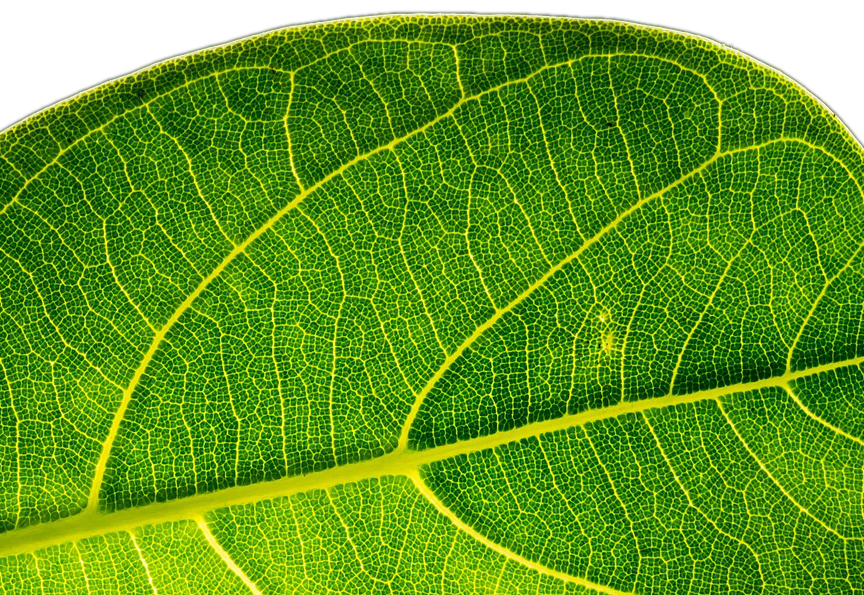
\includegraphics[width=1.0\paperwidth,height=0.5\paperheight]{images/bg}
            };
        \end{tikzpicture}
    }
}
\makeatletter
\def\printauthor{%
    {\large \@author}}
\makeatother

% Set up bibliography
%----------------------------------------------------------------------------
\addbibresource{inc/bibliography.bib}
\DefineBibliographyStrings{ngerman}{
    andothers = {{et\,al\adddot}},
}

\begin{document}

% Title Page and Abstract
%---------------------------------------------------------------------------
\setcounter{page}{1}
% -*- mode: latex; coding: utf-8 -*-

\begin{titlepage}
    \BgThispage
    \begin{fullwidth}%
        \sffamily%
        \fontsize{36}{40}\selectfont\par\noindent\textcolor{darkgray}{\allcaps{\titletext}}
        \vspace{3mm}
        \fontsize{18}{20}\selectfont\par\noindent\textcolor{darkgray}{\allcaps{\subtitletext}}
        \vspace{6mm}
        \fontsize{14}{16}\selectfont\par\noindent\allcaps{\subsubtitletext}%
        \vspace{24mm}
        \normalsize\normalfont%
        \begin{tabbing}
        xxxxxxxxxxxxxxx   \= xxxxxxxxxxxxxxxxxxxxxxxxxxxxxxxxxxxxxxxxxxxxxxx \kill
        Major:            \> Computer science                                         \\
        Author:           \> Sven Osterwalder\protect\footnotemark[1]{}         \\
        Advisor:          \> Prof.~Claude Fuhrer\protect\footnotemark[2]{} \\
        Expert:           \> Dr.~Eric Dubuis\protect\footnotemark[3]{} \\
        Date:             \> \vhCurrentDate{}\\
        Version:          \> \vhCurrentVersion\\
        \end{tabbing}
        \vspace{10mm}
        \begin{tabularx}{0.5\textwidth}{@{}XX@{}}
            
\includegraphics[width=50px]{images/by-sa-big} &
            
\includegraphics[height=20pt]{images/BFH_Logo_B} \\

            \tiny{\sffamily{This work is licensed under
            a~\href{http://creativecommons.org/licenses/by-sa/4.0/}{Creative
            Commons Attribution-ShareAlike 4.0 International
            License}.}}\index{license}
            & \tiny{\sffamily{Berne University of Applied Sciences}}\\
        \end{tabularx}
        \footnotetext[1]{sven.osterwalder@students.bfh.ch}
        \footnotetext[2]{claude.fuhrer@bfh.ch}
        \footnotetext[3]{eric.dubuis@comet.ch}
    \end{fullwidth}%
\end{titlepage}
\restoregeometry
\thispagestyle{empty}%
\clearpage%

% -*- mode: latex; coding: utf-8 -*-

% Versions:
% -----------------------------------------------

\chapter*{}
\label{chap:versions}

\begin{versionhistory}
    \vhEntry{ 89c7544 }{ 2017-02-28 17:09:43 }{ SO }{ Set up initial project structure, provide first content }
    \vhEntry{ 10192d8 }{ 2017-03-02 22:37:17 }{ SO }{ Set up project schedule }
    \vhEntry{ 54f4b23 }{ 2017-03-05 22:53:15 }{ SO }{ Set up project structure, implement main entry point and main window }
    \vhEntry{ ffda0e5 }{ 2017-03-15 10:58:51 }{ SO }{ Scene graph, logging, adapt project schedule }
    \vhEntry{ 34b09b7 }{ 2017-03-24 17:08:22 }{ SO }{ Update meeting minutes, thoughts about node implementation }
    \vhEntry{ 06fe268 }{ 2017-04-03 23:00:35 }{ SO }{ Add requirements, node graph implemenetation }
    \vhEntry{ d264175 }{ 2017-04-10 16:07:01 }{ SO }{ Conversion from Org-Mode to Nuweb, revise editor implementation }
    \vhEntry{ f8b524b }{ 2017-04-30 23:42:57 }{ SO }{ Approach node graph and nodes }
    \vhEntry{ 2f46832 }{ 2017-05-04 21:13:41 }{ SO }{ Impel node definitions further }
    \vhEntry{ ae34fc5 }{ 2017-05-24 13:56:31 }{ SO }{ Change class to tufte-book, title page, introduction, further implementation }
    \vhEntry{ 27c549c }{ 2017-05-24 22:28:41 }{ SO }{ Change document structure, re-work admin. aspects }
    \vhEntry{ 6772ef9 }{ 2017-05-27 14:18:09 }{ SO }{ Adapt document structure, fundamentals: introduction and rendering }
    
\end{versionhistory}% -*- coding: utf-8 -*-

\chapter*{Abstract}
\label{chap:abstract}

\todo[inline]{Provide correct abstract.}
A highly optimized rendering algorithm based on ray
tracing is presented. It outperforms the classical ray tracing methods and
allows the rendering of ray traced scenes in real-time on the GPU.~The
classical approach for modelling scenes using triangulated meshes is replaced
by mathematical descriptions based on signed distance functions. The
effectiveness of the algorithm is demonstrated using a prototype application
which renders a simple scene in real-time.

% Richtet sich der Bericht an eine breitere Öffentlichkeit oder an technische Laien, die aufgrund fehlender
% Sachkenntnis nicht den ganzen Bericht lesen wollen, dann kann die Zusammenfassung zum
% wichtigsten Teil eines Berichts werden [3, p. 24]. Die Zusammenfassung ist der meistgelesene Teil
% einer Publikation. Sie gibt einen Überblick zur Problemstellung, zum Inhalt und zu den Resultaten des
% Berichts. Eine gute Zusammenfassung kann die Leserin, den Leser ermutigen, ausgewählte Teile der
% Arbeit oder den gesamten Bericht zu studieren.
% Die Zusammenfassung muss unabhängig vom Rest der Arbeit verständlich sein und besonders
% schlüssig formuliert werden. Literaturangaben werden in der Zusammenfassung keine gemacht.
% Die Zusammenfassung gehört an den Anfang eines Berichts. Oft wird sie auch mit Abstract oder
% Summary bezeichnet.
% Je nach Länge der Arbeit werden der Auftrag, die Ausgangslage, das Vorgehen und die wesentlichen
% Ergebnisse und Schlussfolgerungen des Berichts im Umfang zwischen einer halben und maximal einer
% ganzen A4-Seite dargelegt. Die eigenen Resultate bilden den inhaltlichen Schwerpunkt der
% Zusammenfassung.
% Die Zusammenfassung wird erst am Ende des Arbeitsprozesses verfasst.

% Table of contents / Lists of
%---------------------------------------------------------------------------
\tableofcontents{}
\listoffigures{}
\listoftables{}

% Main part
%---------------------------------------------------------------------------
\newpage{}
% -*- mode: latex; coding: utf-8 -*-

\chapter{Introduction}
\label{chap:introduction}

% Die Einleitung gibt Antwort auf die Frage, weshalb es den Bericht gibt und wie
% er zustande gekommen ist [3, p. 25]. Im ersten Teil wird das Thema der Arbeit
% eingeführt. Die Relevanz und Aktualität des Themas oder der fachliche Kontext
% der Untersuchung werden dazu kurz umschrieben. Die Einleitung hält explizit
% fest, welchen Auftrag der Bericht erfüllt [3, p. 25]. Der Auftrag muss so klar
% und präzise wie möglich formuliert werden. Auftraggeber und Auftragnehmer werden
% festgehalten. Der zweite Teil der Einleitung stellt den Ist-Zustand oder den
% bisherigen Wissensstand knapp dar. Darauf aufbauend wird das eigene Thema
% eingegrenzt. Es gibt Untersuchungen, bei denen es für das Verständnis wichtig
% ist, den genauen Ist-Zustand zu kennen. Wenn es für ein Projekt bereits ein
% Vorprojekt gibt, auf dessen Resultate der Bericht aufbaut, oder in Bauprojekten
% ist es üblich, die Ausgangslage in einem gesonderten Kapitel zu beschreiben. Im
% dritten Teil wird die präzise Fragestellung formuliert. Das Ziel des Berichts
% wird genannt und es wird erläutert, welchen Nutzen die Untersuchung haben soll.

\newthought{The subject of computer graphics} exists since the beginning of
modern computing. Ever since the subject of computer graphics has strived to
create realistic depictions of the observable reality. Over time various
approaches for creating artificial images (the so called rendering) evolved.
One of those approaches is ray tracing.
It was introduced in~\citeyear{appel_techniques_1968}
by~\citeauthor{appel_techniques_1968} in the
work~\citetitle{appel_techniques_1968}~\cite{appel_techniques_1968}. In
\citeyear{whitted_improved_1980} it was improved
by~\citeauthor{whitted_improved_1980} in his work
\citetitle{whitted_improved_1980}~\cite{whitted_improved_1980}.

\newthought{Ray tracing captivates} through simplicity while providing a very
high image quality including perfect refractions and reflections. For a long
time although, the approach was not performant enough to deliver images in real
time. Real time means being able to render at least 25 rendered images (frames)
within a second. Otherwise, due to the human anatomy, the output is perceived as
either still images or as a too slow animation.

\newthought{Sphere tracing} is a ray tracing approach introduced
in~\citeyear{hart_sphere_1994} by~\citeauthor{hart_sphere_1994} in his
work~\citetitle{hart_sphere_1994}~\cite{hart_sphere_1994}. This approach is
faster than the classical ray tracing approaches in finding intersections
between rays and objects. The speed up is achieved by using signed distance
functions for modeling the objects to be rendered and by expanding volumes for
finding intersections.

\newthought{Graphics processing units (GPUs)} have evolved over time and have
gotten more powerful in processing power. Since around 2009 GPUs are able to
produce real time computer graphics using sphere tracing. While allowing ray
tracing in real time on modern GPUs, sphere tracing has also a clear
disadvantage. The de facto way of representing objects, using triangle based
meshes, cannot be used directly. Instead distance fields defined by implicit functions build the basis for sphere tracing.

\section{Purpose and situation}
\label{sec:purpose}

\subsection{Motivation}
\label{subsec:motivation}

\newthought{To this point in time} there are no solutions (at least none are
known to the author), that provide a convenient way for modeling, animating and
rendering objects and scenes using signed distance functions for modeling and
sphere tracing for rendering.
Most of the solutions using sphere tracing implement it by having one or
multiple big fragment shaders containing everything from modeling to lighting.
Other solutions provide node based approaches, but they allow either no sphere
tracing at all, meaning they use rasterization, or they provide nodes containing
(fragment-) shader code, which leads again to a single big fragment shader.

\newthought{This thesis} aims at designing and developing a software which
provides both: a node based approach for modeling and animating objects using
signed distance functions as well as allowing the composition of scenes while
rendering objects, or scenes respectively, in real time on the GPU using sphere
tracing.

\subsection{Objectives and limitations}
\label{subsec:objectives}

\newthought{The objective of this thesis} is the design and development of a
software for \textit{modeling}, \textit{composing} and \textit{rendering} real
time computer graphics through a graphical user interface.

\newthought{Modeling} is done by composing single nodes to objects using a
node based graph structure.

\newthought{Compositing} includes two aspects: the composition of objects into
scenes and the composition of an animation which is defined by multiple scenes
which follow a chronological order. The first aspect is realized by a scene
graph structure, which contains at least a root scene. Each scene may contain
nodes. The second aspect is realized by a time line, which allows a
chronological organization of scenes.

\newthought{For rendering} a highly optimized algorithm based on ray tracing is
used. The algorithm is called sphere tracing and allows the rendering of ray
traced scenes in real time on the GPU. Contingent upon the used rendering
algorithm all models are modeled using implicit surfaces. In addition
mesh-based models and corresponding rendering algorithms may be implemented.

\newthought{Required objectives} are the following:
\begin{itemize}
  \item Development of an editor for creating and editing real time rendered
    scenes, containing the following features.
    \begin{itemize}
      \item A scene graph, allowing management (creation and deletion) of
        scenes. The scene graph has at least a root scene.
    \item A node-based graph structure, allowing the composition of scenes using
      nodes and connections between the nodes.
    \item Nodes for the node-based graph structure.
      \begin{itemize}
        
        \item Simple objects defined by signed distance functions: Cube and
          sphere
        \item Simple operations: Merge/Union, Intersection, Difference
        \item Transformations: Rotate, Translate and Scale
        \item Camera
        \item Renderer (ray traced rendering using sphere tracing)
        \item Lights
      \end{itemize}
    \end{itemize}
\end{itemize}

\newthought{Optional objectives} are the following:
\begin{itemize}
  \item Additional features for the editor, as follows.
  \begin{itemize}
    \item A sequencer, allowing a time-based scheduling of defined scenes.
    \item Additional nodes, such as operations (e.g. replication of objects)
      or post-processing effects (glow/glare, color grading and so on).
  \end{itemize}
  \item Development of a standalone player application. The player allows the
    playback of animations (time-based, compounded scenes in sequential order)
    created with the editor.
\end{itemize}

\section{Related works}
\label{sec:related-works}

\newthought{Preliminary} to this thesis two project works were done:
\enquote{Volume ray casting --- basics \&
principles}~\cite{osterwalder_volume_2016}, which describes the basics and
principles of sphere tracing, a special form of ray tracing, and \enquote{QDE
--- a visual animation system, architecture}~\cite{osterwalder_qde_2016}, which
established the ideas and notions of an editor and a player component as well as
the basis for a possible software architecture for these components. The latter
project work is presented in detail in the chapter about the procedure, the
former project work is presented in the chapter about the implementation.

\section{Document structure}
\label{sec:document-structure}

This document is divided into six chapters, the first being this \textit{introduction}. The
second chapter on \textit{administrative aspects} shows the planning of the
project, including the involved persons, deliverables and the phases and
milestones.

The administrative aspects are followed by a chapter on the
\textit{fundamentals}. The purpose of that chapter is to present the
fundamentals, that this thesis is built upon. One aspect is a framework for the
implementation of the intended software, which is heavily based on the previous
project work, \enquote{QDE --- a visual animation system, architecture}~\cite{osterwalder_qde_2016}. Another aspect is the rendering,
which is using a special form of ray tracing as described in ``Volume ray
casting --- basics \& principles''~\cite{osterwalder_volume_2016}.

The next chapter on the \textit{methodologies} introduces a concept called
literate programming and elaborates some details of the implementation using
literate programming. Additionally it introduces standards and principles
concerning the implementation of the intended software.

The following chapter on the \textit{results} concludes on the implementation
of the editor and the player components.
% TODO: Elaborate more?

% TODO: Move this to a more fitting place
% ray casting --- basics \& principles''~\cite{osterwalder_volume_2016}. As the
% editor component defines the whole data structure it builds the basis of the
% thesis and can be seen as main part of the thesis. The player component re-uses
% concepts established within the editor.
% Given that literate programming is very complete and elaborated, as components
% being developed using this procedure are completely derived from the
% documentation, the actual implementation is found in the appendix as otherwise
% this thesis would be simply too extensive.

The last chapter is \textit{discussion and conclusion} and discusses the
methodologies as well as the results. Some further work on the editor and the
player components is proposed as well.

After the regular content follows the \textit{appendix}, containing the
requirements for building the before mentioned components, the actual source
code in form of literal programming as well as test cases for the components.
% TODO: Add missing content, if content _is_ missing.
% -*- mode: latex; coding: utf-8 -*-

\chapter{Administrative aspects}
\label{chap:administrative_aspects}

% Link to previous
% Make a connection to what has immediately gone before. Recap the last chapter.
% In the last chapter I showed that… Having argued in the previous chapter that…
% As a result of x, which I established in the last chapter….. It is also possible
% to make a link between this chapter and the whole argument… The first step in
% answering my research question (repeat question) .. was to.. . In the last
% chapter I …
\newthought{The last chapter} provided an introduction to this thesis by
outlining the purpose and situation, the related works and the document
structure.

% Focus: What does this chapter specifically do?
% Now focus the reader’s attention on what this chapter is specifically going to
% do and why it is important. In this chapter I will examine.. I will present… I
% will report … This is crucial in (aim of thesis/research question) in order to….
\newthought{This chapter} covers some administrative aspects of this thesis,
they are although not required for understanding of the result.

% Overview: How is it done?
% The third paragraph simply outlines the way that you are going to achieve the
% aim spelled out in the previous paragraph. It’s really just a statement of the
% contents in the order that the reader will encounter them. It is important to
% state these not simply as topics, but actually how they build up the internal
% chapter argument… I will begin by examining the definitions of, then move to
% seeing how these were applied… I first of all explain my orientation to the
% research process, positioning myself as a critical scholar.. I then explain the
% methodology that I used in the research, arguing that ethnography was the most
% suitable approach to provide answers to the question of…
\newthought{The first section} defines the involved persons and their role
during this thesis. Afterwards the deliverable items are shown and described.
The last section elaborates on the organization of work including meetings, the
phases and milestones as well as the thesis's schedule.

\newthought{Note that} the whole documentation uses the male form, whereby both
genera are equally meant.

\section{Involved persons}
\label{sec:involved_persons}

\begin{table}[h]
  \caption{List of the involved persons.}
  \begin{tabularx}{\textwidth}{llX}
    \toprule
    \textbf{Role} & \textbf{Name} & \textbf{Task} \\
    \midrule
    \textit{Author}  & Sven Osterwalder\protect\footnotemark[1]{} & Author of the thesis.\\
    \textit{Advisor} & Prof.\ Claude Fuhrer\protect\footnotemark[2]{} & Supervises the student doing the thesis.\\
    \textit{Expert}  & Dr.\ Eric Dubuis\protect\footnotemark[3]{}     & Provides expertise concerning the thesis's subject, monitors and grades the thesis.\\
    \bottomrule
  \end{tabularx}
\end{table}
\footnotetext[1]{sven.osterwaldertudents.bfh.ch}
\footnotetext[2]{claude.fuhrer@bfh.ch}
\footnotetext[3]{eric.dubuis@comet.ch}

\newpage{}

\section{Deliverables}
\label{sec:deliverables}

\begin{table}[h]
  \caption{List of deliverables.}
  \begin{tabularx}{\textwidth}{lX}
    \toprule
    \textbf{Deliverable} & \textbf{Description} \\
    \midrule
    \textit{Report} & The report contains the theoretical and technical details for
    implementing a system for composing real time computer graphics. \\
    \midrule
    \textit{Implementation} & The implementation of a system for composing real time
    computer graphics, which was developped during this thesis. \\
    \bottomrule
  \end{tabularx}
\end{table}

\section{Organization of work}
\label{sec:organization-of-work}

\subsection{Meetings}
\label{subsec:meetings}

\newthought{Various meetings} with the supervisor and the expert helped reaching
the defined goals and preventing erroneous directions of the thesis. The
supervisor and the expert supported the author of this thesis by providing
suggestions throughout the held meetings. The minutes of the meetings may be
found under meeting minutes. \todo[inline]{Add correct reference}

\subsection{Phases and milestones}
\label{subsec:project-phases-milestones}

\begin{table}[h]
  \caption{Phases of the project.}
  \begin{tabularx}{\textwidth}{Xr}
    \toprule
    \textbf{Phase}   & \textbf{Week / 2017} \\
    \midrule
    Start of the project & 8 \\
    Definition of objectives and limitation & 8-9 \\
    Documentation and development & 8-30 \\
    Corrections & 30-31 \\
    Preparation of the thesis' defense & 31-32 \\
    \bottomrule
  \end{tabularx}
\end{table}

\begin{table}[h]
  \caption{Milestones of the project.}
  \begin{tabularx}{\textwidth}{Xr}
    \toprule
    \textbf{Milestone}   & \textbf{End of week / 2017} \\
    \midrule
    Project structure is set up & 8 \\
    Mandatory project goals are reached & 30 \\
    Hand-in of the thesis & 31 \\
    Defense of the thesis & 32 \\
    \bottomrule
  \end{tabularx}
\end{table}

\newpage{}

\subsection{Schedule}
\label{subsec:project-schedule}

\begin{figure*}[ht]
    \begin{ganttchart}[
        vgrid,
        x unit=4.5mm,
        y unit chart=0.87cm,
        bar/.append style={fill=bfhgrey!50},
    ]{1}{26}
        \gantttitle{2017}{26} \ganttnewline{}
        \gantttitlelist{7,...,32}{1} \ganttnewline{}
        \ganttbar{Start of the project}{1}{1} \ganttnewline{}
        \ganttmilestone{Project is set up}{1} \ganttnewline{}
        \ganttlinkedbar{Objectives and limitations}{2}{3} \ganttnewline{}
        \ganttlinkedbar{Documentation}{3}{23} \ganttnewline{}
        \ganttbar{Development}{3}{23} \ganttnewline{}
        \ganttmilestone{Goals reached}{23} \ganttnewline{}
        \ganttlinkedbar{Corrections}{23}{24} \ganttnewline{}
        \ganttmilestone{Hand-in}{24} \ganttnewline{}
        \ganttlinkedbar{Thesis' defense preparation}{25}{26} \ganttnewline{}
        \ganttmilestone{Thesis defense}{26}
    \end{ganttchart}
    \caption{Schedule of the project. The subtitle displays calendar weeks.}
\end{figure*}
% -*- mode: latex; coding: utf-8 -*-

\chapter{Fundamentals}
\label{chap:fundamentals}

% Der aktuelle Wissensstand zum behandelten Thema oder zur Fragestellung muss zu
% Beginn der Arbeit beschrieben werden. Die Vorarbeiten und Publikationen, auf die
% sich der Bericht stützt, werden genannt [3, p. 26]. Je nach Arbeit und
% Zielpublikum werden die Grundlagen kurz zusammengefasst und einander
% gegenübergestellt. Der theoretische Hintergrund oder Normen, die für die
% Untersuchung eine Rolle spielen, werden objektiv dargestellt. Gibt es nur sehr
% wenige Grundlagen, die eingangs der Arbeit erläutert werden müssen, können diese
% Informationen auch als Absatz in der Einleitung oder als Unterkapitel zum
% Kapitel der Einleitung verfasst werden.

% Link to previous
% Make a connection to what has immediately gone before. Recap the last chapter.
% In the last chapter I showed that… Having argued in the previous chapter that…
% As a result of x, which I established in the last chapter….. It is also possible
% to make a link between this chapter and the whole argument… The first step in
% answering my research question (repeat question) .. was to.. . In the last
% chapter I …
\newthought{The last chapter} covered some administrative aspects including the
involved persons, the phases and milestones of the thesis as well as its
schedule.

% Focus: What does this chapter specifically do?
% Now focus the reader’s attention on what this chapter is specifically going to
% do and why it is important. In this chapter I will examine.. I will present… I
% will report … This is crucial in (aim of thesis/research question) in order to….
\newthought{This chapter} presents the fundamentals which are required for
understanding of the result of this thesis.

% Overview: How is it done?
% The third paragraph simply outlines the way that you are going to achieve the
% aim spelled out in the previous paragraph. It’s really just a statement of the
% contents in the order that the reader will encounter them. It is important to
% state these not simply as topics, but actually how they build up the internal
% chapter argument… I will begin by examining the definitions of, then move to
% seeing how these were applied… I first of all explain my orientation to the
% research process, positioning myself as a critical scholar.. I then explain the
% methodology that I used in the research, arguing that ethnography was the most
% suitable approach to provide answers to the question of…
\newthought{The first section of this chapter} defines the software architecture
that is used for the implementation of the intended software. It is mainly a
summary of the previous project work,~\enquote{QDE --- a visual animation
system, architecture}~\cite{osterwalder_qde_2016}. The second section shows the
algorithm which is used for rendering. It is a summary of a previous project
work,~\enquote{Volume ray casting --- basics \&
principles}~\cite{osterwalder_volume_2016}.

\section{Software architecture}
\label{sec:architecture}

\newthought{``An architecture is the \textit{set of significant
decisions}} about the organization of a software system, the selection of
\textit{structural elements} and their interfaces by which the system is
composed, together with their \textit{behavior} as specified in the
collaborations among those elements, the \textit{composition} of these elements
into progressively larger subsystems, and the \textit{architectural style} that
guides this organization -- these elements and their interfaces, their
collaborations, and their composition.''~\cite{kruchten_rup_2003}

Or as~\citeauthor{fowler_architect_2003} puts it:~\enquote{Whether something
is part of the architecture is entirely based on whether the developers think it
is important. [...] So, this makes it hard to tell people how to describe their
architecture.~\enquote{Tell us what is important.} Architecture is about the
important stuff. Whatever that is.}~\cite{fowler_architect_2003}

\newthought{This~\autoref{sec:architecture}} is a summary of the previous
project work of the author,~\enquote{QDE --- a visual animation system,
architecture}~\cite{osterwalder_qde_2016}. It describes the fundamentals for the
architecture for the intended software of this thesis.

\section{Rendering}
\label{sec:rendering}

\newthought{This~\autoref{sec:rendering}} is a summary of a previous project
work of the author,~\enquote{Volume ray casting --- basics \&
principles}~\cite{osterwalder_volume_2016}. It describes the fundamentals for
the rendering algorithm that is used for the intended software of this thesis.

\newthought{Rendering} is one of the main aspects of this thesis, as the main
objective of the thesis is the design and development of a software for
modeling, composing and \textit{rendering} real time computer graphics through a
graphical user interface. \citeauthor{foley_computer_1996} describes rendering
as a~\enquote{process of creating images from
models}~\cite{foley_computer_1996}. The basic idea of rendering is to determine
the color of a surface at a certain point. For this task two concepts have
evolved: \textit{illumination models} and \textit{shading models}.
\newthought{Shading models} define when to use which illumination model and the
parameters for the illumination model.

\newthought{Illumination models} describe the amount of light that is
transmitted from a point on a surface to a viewer. There exist two kinds of
illumination models: local illumination models and global illumination models.
Whereas local illumination models aggregate local data from adjacent surfaces
and directly incoming light, global illumination models consider also indirect
light. The algorithm used for rendering in the intended software is an
algorithm using a \textit{global illumination model}.

\newthought{Global illumination models}~\enquote{express the light being
transferred from one point to another in terms of the intensity of the light
emitted from the first point to the second}~\cite[pp. 775 and
776]{foley_computer_1996}. Additionally to this direct intensity the indirect
intensity is considered, therefore ~\enquote{the intensity of light emitted from
all other points that reaches the first and is reflected from the first to the
second}~\cite[pp. 775 and 776]{foley_computer_1996} point is added.

\newthought{In 1986 James~\enquote{Jim}~Kajiya} set up the so called rendering
equation, which expresses this behavior.~\parencites{kajiya_rendering_1986}[p.
776]{foley_computer_1996}

\begin{figure}
  \label{eq:rendering-equation}
  \caption[][-120pt]{The rendering equation as defined by James Kajiya.}
  \begin{equation}
    I(x, x') = g(x, x')[\varepsilon(x, x') + \int\limits_{S}\rho(x, x', x'')I(x', x'')dx'']
  \end{equation}
\end{figure}

\marginnote[-130pt]{%
  \begin{description}
    \item[$x, x' \text{and } x''$] Points in space.
    \item[$I(x, x')$] Intensity of the light going from point $x'$ to point $x$.
    \item[$g(x, x')$] A geometrical term.
      \begin{description}
        \item[$0$] $x$ and $x'$ are occluded by each other.
        \item[$1\over{r^2}$] $x$ and $x'$ are visible to one other, $r$ being
          the distance between the two points.
      \end{description}
    \item[$\varepsilon(x, x')$] Intensity of the light being emitted from point
      $x'$ to point $x$.
    \item[$\rho(x, x', x'')$] Intensity of the light going from $x''$ to $x$, being
      scattered on the surface of point $x'$.
    \item[$\int\limits_{S}$] Integral over the union of all surfaces, hence $S =
      \bigcup\limits_{i=0}^{n} S_{i}$, $n$ being the number of surfaces.
      All points $x$, $x'$ and $x''$ brush all surfaces of all objects within
      the scene. $S_{0}$ being an additional surface in form of a hemisphere
      which spans the whole scene and acts as background.
  \end{description}
}

% \begin{table}[h]
%   \caption{Description of the single aspects of the rendering equation.}
%   \begin{tabularx}{\textwidth}{lX}
%     \toprule
%     \textbf{Part} & \textbf{Description} \\
%     \midrule
%     $x, x' \text{and } x''$ & Points in space. \\
%     \midrule
%     $I(x, x')$ & Intensity of the light going from point $x'$ to point $x$. \\
%     \midrule
%     $g(x, x')$ & A geometrical term. \newline
%         \hspace*{4mm} $0$: \hspace*{2mm} $x$ and $x'$ are occluded by each other.
%         \newline
%         \hspace*{4mm} $1\over{r^2}$: \hspace*{1mm} $x$ and $x'$ are visible to one
%         other, $r$ being the \newline
%         \hspace*{12mm} distance between the two points. \\
%     \midrule
%     $\varepsilon(x, x')$ & Intensity of the light being emitted from point $x'$
%     to point $x$. \\
%     \midrule
%     $\rho(x, x', x'')$ & Intensity of the light going from $x''$ to $x$, being
%     scattered on the surface of point $x'$. \\
%     \midrule
%     $\int\limits_{S}$ & Integral over the union of all surfaces, hence $S =
%     \bigcup\limits_{i=0}^{n} S_{i}$, $n$ being the number of
%     surfaces.
%     All points $x$, $x'$ and $x''$ brush all surfaces of all objects within the
%     scene. $S_{0}$ being an additional surface in form of a hemisphere which
%     spans the whole scene and acts as background.\\
%     \bottomrule
%   \end{tabularx}
% \end{table}

\newthought{Implementing a global illumination model} or the rendering equation
directly for rendering images in viable or even real time is not really
feasible, even on modern hardware. The procedure is computationally complex and
very time demanding.

\newthought{A simplified approach} to implement global illumination models (or
the rendering equation) is ray tracing. Ray tracing is able to produce high
quality, realistic looking images. Although it is still demanding in terms of
time and computations, the time complexity is reasonable for producing still
images. For producing images in real time however, the procedure is still too
demanding. This is where a special form of ray tracing comes in.

\newthought{Sphere tracing} is a ray tracing approach for implicit surfaces
introduced in~\citeyear{hart_sphere_1994} by~\citeauthor{hart_sphere_1994} in
his work~\citetitle{hart_sphere_1994}~\cite{hart_sphere_1994}. 
Sphere tracing is faster than the classical ray tracing approaches in finding
intersections between rays and objects. In contrast to the classical ray tracing
approaches, the marching distance on rays is not defined by an absolute or a
relative distance, instead distance functions are used. The distance functions
are used to expand unbounding volumes (in this concrete case spheres, hence the
name) along rays.~\autoref{fig:} illustrates this procedure.

\begin{figure}[h]
    \caption{Illustration of the sphere tracing
      algorithm.
      Ray~\textit{e} hits no objects until reaching the horizon at
      $d_{max}$. Rays~\textit{f},~\textit{g} and~\textit{h} hit
      polygon~\textit{poly1}.
      \protect\footnotemark}\label{fig:sphere_tracing_1}
    \centering
    \includegraphics{images/sphere_tracing_principle}
\end{figure}
\footnotetext{Own illustration using Inkscape.}

\newthought{Unbounding volumes} contrast with bounding volumes, which enclose a
solid. Unbounding volumes enclose a part of space without including certain
objects (whereas including means touching). For calculating a unbounding volume,
the distance between an object and the origin is being searched. Is this
distance known, it can be taken as a radius of a sphere. Sphere tracing defines
objects as implicit surfaces using distance functions. Therefore the distance
from every point in space to every other point in space and to every surface of
every object is known. These distances build a so called distance field.

\newthought{The sphere tracing algorithm} is as follows. A ray is being shot
from a viewer (an eye or a pinhole camera) through the image plane into a scene.
The radius of an unbounding volume in form of a sphere is being calculated at
the origin, as described above. This radius builds an intersection with the ray
and represents the distance, that the ray will travel in a first step. From this
intersection the next unbounding volume is being expanded and its radius is
being calculated, which gives the next intersection with the ray. This procedure
continues until an object is being hit or until a predefined maximum distance of
the ray $d_{max}$ is being reached. An object is being hit, whenever the
returned radius of the distance function is below a predefined constant
$\epsilon$. A possible implementation of the sphere tracing algorithm is shown
in~\autoref{alg:sphere_tracing}.

 \begin{figure}
   \caption{An abstract implementation of the sphere tracing algorithm\protect\footnotemark.}
   \begin{minted}{python}
def sphere_trace():
    ray_distance          = 0
    estimated_distance    = 0
    max_distance          = 9001
    convergence_precision = 0.000001

    while ray_distance < max_distance:
        # sd_sphere is a signed distance function defining the implicit surface
        # cast_ray defines the ray equation given the current traveled /
        # marched distance of the ray
        estimated_distance = sd_sphere(cast_ray(ray_distance))

        if estimated_distance < convergence_precision:
            # the estimated distance is already smaller than the desired
            # precision of the convergence, so return the distance the ray has
            # travelled as we have an intersection
            return ray_distance

        ray_distance = ray_distance + estimated_distance

    # When we reach this point, there was no intersection between the ray and a
    # implicit surface, so simply return 0
    return 0
   \end{minted}
\end{figure}
\footnotetext{Algorithm in pseudo code, after~\cite{hart_sphere_1994}[S. 531, Fig. 1]}% -*- mode: latex; coding: utf-8 -*-

\chapter{Methodologies}
\label{chap:methodologies}

\todo[inline]{Write chapter.}

% Das Kapitel der Methoden erklärt, was (Material) untersucht wurde und wie
% (Methode) ersteres untersucht wurde. Aufgrund der Beschreibung der Methoden muss
% es möglich sein, den Versuch oder die Studie zu wiederholen. Ist die
% Beschreibung der Versuchsanordnung oder des Vorgehens von sehr geringem Umfang,
% können diese nach Rücksprache mit der Betreuungsperson auch als Absatz in der
% Einleitung oder als Unterkapitel zum Kapitel der Einleitung verfasst werden.% -*- mode: latex; coding: utf-8 -*-

\chapter{Results}
\label{chap:results}

\todo[inline]{Write chapter.}

% Gestützt auf Quellen, Messungen und Datenerhebungen werden die anhand der
% Fragestellung gewon- nenen Ergebnisse präsentiert [3, p. 116]. Während das
% Kapitel zu Material und Methoden ( 3.2.3) oder das entsprechende Unterkapitel
% der Einleitung die Versuchsanordnung beschreibt, werden im Kapitel Ergebnisse
% der Versuchsablauf mit den Resultaten objektiv wiedergegeben. Alle Überlegungen,
% Berechnungen oder Experimente des Berichts müssen vollständig nachvollziehbar
% sein [3, p. 26]. Zusammen mit der Diskussion und den Folgerungen machen die
% Ergebnisse qualitativ und quantitativ den Hauptteil des Berichts aus [3, p. 26].% -*- mode: latex; coding: utf-8 -*-

\chapter{Discussion and conclusion}
\label{chap:discussion-conclusion}

\todo[inline]{Write chapter.}

% Im Kapitel Diskussion setzt sich die Autorin, der Autor mit den erzielten
% Ergebnissen auseinander. Diese werden interpretiert und mit Erkenntnissen aus
% anderen Studien zur gleichen Fragestellung beurteilt. Die Diskussion schafft die
% nötigen Grundlagen, damit die in der Einleitung formulierte Fragestellung
% möglichst gut und sachlich richtig beantwortet werden kann.

% In den Folgerungen können die wichtigsten Ergebnisse in ihrer kritischen
% Würdigung prägnant zusammengefasst werden. Es wird eine Art Schlussbilanz
% gezogen. Aus der detaillierten Darstellung der Ergebnisse und deren Diskussion
% lässt sich in der Regel eine Antwort auf die Ausgangsfrage ableiten [3, p. 26].
% Die Antwort auf die Fragestellung kann zu Empfeh- lungen für die Ausführung in
% der Praxis oder für weitere Studien führen. Die Folgerungen dürfen keine neuen
% Elemente und Aspekte enthalten, welche nicht schon in den Ergebnissen und in der
% Diskussion behandelt wurden. Wenn die Problemstellung der Arbeit nur sehr wenige
% Folgerungen verlangt, können diese auch als Schlussteil in die Diskussion
% integriert werden.
% TODO: Check if still needed
% i inc/procedure.w
% i inc/implementation.w


% Backmatter
%---------------------------------------------------------------------------
\backmatter{}

% Appendix
% i inc/appendix.w
\todo[inline]{fix appendix}

% Bibliography
\printbibliography{}

% Glossary
% \cleardoublepage{}
% \phantomsection{}
% \addcontentsline{toc}{chapter}{Glossary}
% \glsaddall{}
% \printglossaries{}
\todo[inline]{Fix glossaries}

% Index
% \printindex{}
\todo[inline]{Print index}

\end{document}
